\documentclass[specialist, subf, href, colorlinks=true, 12pt, times, mtpro, final]{disser}
\usepackage [russian] {babel}
\usepackage [utf8] {inputenc}
\usepackage {amsmath}
\usepackage {amsthm}
\usepackage {amssymb}
\usepackage{wrapfig}
\usepackage{enumitem}
\usepackage{amsfonts}
\usepackage{textcomp}
\usepackage{graphicx}
\usepackage{float}
\usepackage{caption}
\usepackage{algorithm}
\usepackage{xcolor}
\usepackage{hyperref}
\usepackage{pdfpages}
\usepackage{dsfont}
\usepackage{upgreek}

\theoremstyle{definition}
\newtheorem{defn}{Определение}[section]
\newtheorem{example}{Пример}[section]
\newtheorem{state}{Утверждение}[section]
\newtheorem{theorem}{Теорема}[section]
\newtheorem{lemma}{Лемма}[section]
\newtheorem{axiom}{Аксиома}[section]
\newtheorem{consequence}{Следствие}[section]

\definecolor{linkcolor}{HTML}{0000FF}
\definecolor{urlcolor}{HTML}{0000FF}
\definecolor{faded}{gray}{0.6}

\def\note{\textcolor{faded}}
\def\rk{\text{rank}}
\def\span{\text{span}}
\def\const{\text{const}}
\def\Ker{\text{Ker}}

%---------------------------- defines for bold letters ----------------------------
%                             ( use in mathmode only )
\def\bfa{\mathbf{a}}
\def\bfb{\mathbf{b}}
\def\bfc{\mathbf{c}}
\def\bfd{\mathbf{d}}
\def\bfe{\mathbf{e}}
\def\bff{\mathbf{f}}
\def\bfg{\mathbf{g}}
\def\bfh{\mathbf{h}}
\def\bfi{\mathbf{i}}
\def\bfj{\mathbf{j}}
\def\bfk{\mathbf{k}}
\def\bfl{\mathbf{l}}
\def\bfm{\mathbf{m}}
\def\bfn{\mathbf{n}}
\def\bfo{\mathbf{o}}
\def\bfp{\mathbf{p}}
\def\bfq{\mathbf{q}}
\def\bfr{\mathbf{r}}
\def\bfs{\mathbf{s}}
\def\bft{\mathbf{t}}
\def\bfu{\mathbf{u}}
\def\bfv{\mathbf{v}}
\def\bfw{\mathbf{w}}
\def\bfx{\mathbf{x}}
\def\bfy{\mathbf{y}}
\def\bfz{\mathbf{z}}

\def\bfA{\mathbf{A}}
\def\bfB{\mathbf{B}}
\def\bfC{\mathbf{C}}
\def\bfD{\mathbf{D}}
\def\bfE{\mathbf{E}}
\def\bfF{\mathbf{F}}
\def\bfG{\mathbf{G}}
\def\bfH{\mathbf{H}}
\def\bfI{\mathbf{I}}
\def\bfJ{\mathbf{J}}
\def\bfK{\mathbf{K}}
\def\bfL{\mathbf{L}}
\def\bfM{\mathbf{M}}
\def\bfN{\mathbf{N}}
\def\bfO{\mathbf{O}}
\def\bfP{\mathbf{P}}
\def\bfQ{\mathbf{Q}}
\def\bfR{\mathbf{R}}
\def\bfS{\mathbf{S}}
\def\bfT{\mathbf{T}}
\def\bfU{\mathbf{U}}
\def\bfV{\mathbf{V}}
\def\bfW{\mathbf{W}}
\def\bfX{\mathbf{X}}
\def\bfY{\mathbf{Y}}
\def\bfZ{\mathbf{Z}}
 % defines \bf? macro for \mathbf{?}

\def\bfrd{\dot{\bfr}}
\def\bfrdd{\ddot{\bfr}}
\def\bfqd{\dot{\bfq}}
\def\bfqdd{\ddot{\bfq}}

\def\bfalpha{\upalpha}
\def\bfbeta{\upbeta}
\def\bfphi{\upphi}
\def\bfomega{\mathbf{\omega}}
\def\bfrho{\mathbf{\rho}}

\def\bfzero{\mathbf{0}}
%----------------------------------------------------------------------------------

\hypersetup{pdfstartview = FitH, linkcolor = linkcolor, urlcolor = urlcolor, colorlinks = true}

\begin{document}
    
    %\tableofcontents

    \section*{Список вопросов}
    %\note{В этом списке нужно расставить ссылки. Или оглавление сделать. Но так имхо удобнее, т.к. сюда можно по оглавлению возвращаться.}
    \begin{enumerate}
    \item \hyperref[1]{Свободная механическая система. Механическая система со связями. Аксиома освобождения от связей. Силы реакции связей. Уравнения связей. Пространство виртуальных скоростей. Принцип Даламбера – Лагранжа. Уравнения Лагранжа первого рода. Идеальные связи.}
    \item \hyperref[2]{Понятие об интегрируемости связей. Критерий интегрируемости (критерий Фробениуса, без доказательства). Обобщенные координаты системы с интегрируемыми связями. Уравнения дифференциальных связей в обобщенных координатах. Признак неинтегрируемости уравнений связей.}
    \item \hyperref[3]{Принцип Даламбера – Лагранжа в обобщенных координатах. Уравнения Лагранжа второго рода для голономных систем. Обобщенные силы. Работа сил на перемещении вдоль координатной линии. Случай потенциальных сил. Уравнения Лагранжа со множителями в обобщенных координатах.}
    \item \hyperref[4]{Энергия ускорений. Псевдоскорости. Уравнения Аппеля.}
    \item \hyperref[5]{Теоремы об изменении импульса, кинетического момента и кинетической энергии для систем со связями и следствия из них.}
    \item \hyperref[6]{Эквивалентность принципа Даламбера – Лагранжа и уравнений движения свободного твердого тела.}
    \item \hyperref[7]{Уравнения Лагранжа второго рода. Калибровка. Преобразование уравнений при замене координат.}
    \item \hyperref[8]{Первые интегралы уравнений Лагранжа для систем с потенциальными силами:
    интеграл Якоби, интеграл энергии, циклические интегралы. Поле симметрий. Теорема Нетер.}
    \item \hyperref[9]{Понижение порядка уравнений Лагранжа по Раусу. Функция Рауса. Приведенный потенциал. Уравнения Рауса.}
    \item \hyperref[10]{Задача Лагранжа о вращении тяжелого твердого тела вокруг неподвижной точки. Типичное движение оси динамической симметрии. Псевдорегулярная и регулярная прецессии. Способы реализации движений этих типов с заданным углом нутации.}
    \item \hyperref[11]{Равновесия системы уравнений Лагранжа. Соответствующие движения механической системы. Уравнения равновесия. Устойчивость равновесий по Ляпунову. Теорема Лагранжа – Дирихле о достаточном условии устойчивости равновесия.}
    \item \hyperref[12]{Линеаризация уравнений Лагранжа в окрестности состояния равновесия. Существование нормальных координат. Линеаризованные уравнения в нормальных координатах, их интегрирование. Уравнение для собственных чисел. Независимость собственных чисел от выбора координат. Собственные векторы. Выражение матрицы преобразования к нормальным координатам через компоненты собственных векторов.}
    \item \hyperref[13]{Преобразование уравнений Лагранжа в уравнения Гамильтона. Обобщенные импульсы. Явный вид функции Гамильтона для уравнений механики.}
    \item \hyperref[14]{Первые интегралы уравнений Гамильтона. Скобки Пуассона в канонических координатах. Свойства скобок Пуассона, тождество Якоби. Простейшие первые интегралы в случаях независимости функции Гамильтона от времени, наличия циклических координат, отделения переменных.}
    \item \hyperref[15]{Аналог теоремы Нетер для уравнений Гамильтона. Теорема о скобке Пуассона двух первых интегралов. Скобки Пуассона компонент кинетического момента свободной точки.}
    \item \hyperref[16]{Канонические преобразования. Определение, его переформулировка в терминах скобок Пуассона, интерпретация в случае системы с одной степенью свободы.
    Примеры: тождественное, обратное к каноническому, ортогональное преобразование фазовой плоскости, полярные канонические координаты, каноническая перестановка, каноническое изменение масштабов на координатных осях.}
    \item \hyperref[17]{Критерии каноничности преобразования.}
    \item \hyperref[18]{Преобразование уравнений Гамильтона при канонических преобразованиях.}
    \item \hyperref[19]{Производящие функции канонических преобразований (свободного и стандартного). Выражение новой функции Гамильтона через производящие функции в этих случаях.
    Производящие функции для преобразований: тождественного, перехода к полярным каноническим координатам, канонической перестановки, канонического изменения масштабов на координатных осях.}
    \item \hyperref[20]{Уравнения для производящих функций целенаправленных канонических преобразований. Уравнение Гамильтона – Якоби, его полный интеграл. Теорема Якоби. Нахождение полного интеграла в случаях независимости функции Гамильтона от времени, наличия циклических координат, отделения переменных.}
    \item \hyperref[21]{Теорема Лиувилля об интегрировании в квадратурах системы уравнений Гамильтона.}
    \item \hyperref[22]{Канонические отображения в фазовом пространстве в канонических координатах. Каноничность отображения вдоль решений системы уравнений Гамильтона. Сохранение фазового объема при этом отображении. Интегральный инвариант Пуанкаре.}
    \item \hyperref[23]{Интегральный инвариант Пуанкаре – Картана.}
    \item \hyperref[24]{Вариационный принцип Гамильтона в фазовом пространстве системы уравнений Гамильтона.}
    \item \hyperref[25]{Вариационный принцип Гамильтона на конфигурационном многообразии системы уравнений Лагранжа.}
    \item \hyperref[26]{Метод усреднения для систем Гамильтона в стандартной форме. Математический маятник с точкой подвеса, движущейся по эллипсу.}
    \end{enumerate}

    \section{Свободная механическая система. Механическая система со связями. Аксиома освобождения от связей. Силы реакции связей. Уравнения связей. Пространство виртуальных скоростей. Принцип Даламбера – Лагранжа. Уравнения Лагранжа первого рода. Идеальные связи.}
    \label{1}
    \hyperlink {first_lects.1}{Лекции}
    \begin{defn} (\hyperlink{first_lects.1}{Свободная механическая система})\\
    {\it Свободная механическая система} -- система $(m_i, \bfr_i)_{i=1}^N$,\ 
    $\bfr_i = (x_i, y_i, z_i)^T$, движущаяся под действием $\bfF = \left((\bfF_i^T)_{i=1}^N\right)^T
    = \bfF(t,\bfr,\bfrd)$, где $\bfr = \left((\bfr_i^T)_{i=1}^N\right)^T$.
    \end{defn}
    \begin{theorem} (\hyperlink{first_lects.1}{Второй закон Ньютона})\\
    Пусть $\bfr=\bfr(t)$ -- движение $(m_i, \bfr_i)_{i=1}^N$ под действием $\bfF$,
    и $M\bfrdd(t_0) = \bfF|_{\bfr = \bfr(t), \bfrd=\bfrd(t)}|_{t=t_0}$, где
    $M = \text{diag}(m_iE_3)_{i=1}^N$. Тогда $\forall t \in \mathbb{R}$:
    $$M\bfrdd(t) = \bfF|_{\bfr=\bfr(t), \bfrd = \bfrd(t)}.$$
    \end{theorem}
    \begin{defn} (\hyperlink{first_lects.1}{Механическая система со связями})\\
    {\it Механическая система со связями} -- система $(m_i, \bfr_i)_{i=1}^N$, движущаяся под
    действием $\bfF$ с ограничениями на $\bfr$ и $\bfrd$.
    \end{defn}
    \begin{axiom} (\hyperlink{first_lects.1}{Освобождения от связей})\\
    Пусть $\bfr=\bfr(t)$ -- движение $(m_i, \bfr_i)_{i=1}^N$ под действием $\bfF$ со
    связями. Тогда $\exists\  \bfR=\left((\bfR_i^T)_{i=1}^N\right)^T = \bfR(t,\bfr,\bfrd)$,
    что из $M\bfrdd(t_0) = (\bfF + \bfR)|_{\bfr = \bfr(t), \bfrd=\bfrd(t)}|_{t=t_0}$
    следует, что
    $$\forall t \in \mathbb{R}\ \ \ M\bfrdd(t) = (\bfF + \bfR)|_{\bfr = \bfr(t), \bfrd=\bfrd(t)}.$$
    $\bfR$ называется {\bf силами реакции связей}.
    \end{axiom}
    \noindent{\bf Уравнения связей.}\\
    $\{(\bfr^T, \bfrd^T)^T\}$ -- {\it фазовое пространство.}\\
    $\{(t, \bfr^T, \bfrd^T)^T\}$ -- {\it расширенное фазовое пространство.}\\
    Будем считать, что $\forall (t_0, \bfr_0^T, \bfrd_0^T)^T \ \ \exists!$ решение
    $M\bfrdd = \bfF + \bfR$:\\ $\bfr(t_0) = \bfr_0,\ \bfrd(t_0) = \bfrd_0$.\\
    Далее будем рассматривать {\bf связи, линейные по $\bfrd$}.
    $$
    \boxed{
    A\bfrd + \bfa = \bfzero},
    $$
    где $A=A(t,\bfr)\in\text{GL}(\mathbb{R}^k, \mathbb{R}^{3N}),\ \ \bfa=\bfa(t,\bfr)\in\mathbb{R}^k,\ \ \rk(A) = k < 3N$.\\
    \note{(жирным нулем здесь и далее обозначается вектор из нулей)}\\
    \noindent\hyperlink{first_lects.2}{Пример (низ страницы).}\\
    $\bfr\in\mathbb{R}^{3N},\ \ \bfrd, \bfF, \bfR,... \in T_{\bfr}\mathbb{R}^{3N}$,
    $N_{\bfr} = \span\{a_j\}_{j=1}^k$.
    \begin{defn} (\hyperlink{first_lects.3}{Пространство виртуальных скоростей})\\
    $L_{\bfr} = N_{\bfr}^T = \{\bfv\in\mathbb{R}^{3N}:\ A\bfv=\bfzero\} = \text{Ker}(A),$\\
    $\dim N_{\bfr} = k$,\,\, $\dim L_{\bfr} = 3N-k$,\,\,  $T_{\bfr}\mathbb{R}^{3N} = N_{\bfr}\oplus L_{\bfr}$.
    \end{defn}
    \noindent\hyperlink{first_lects.3}{(его свойства тут)}
    \begin{theorem} (\hyperlink{first_lects.3}{Принцип Даламбера-Лагранжа})\\
    $\bfr=\bfr(t)$ -- движение $(m_i, \bfr_i)_{i=1}^N$ под действием $\bfF$ со
    связями $A\bfrd+\bfa=\bfzero$ $\Longleftrightarrow\,\,\,\forall t\in\mathbb{R}:\,$\\
    $\left[ \forall\bfv\in\text{Ker}(A)|_{\bfr=\bfr(t)}:\ \langle M\bfrdd(t)-\bfF-\bfR_L,\bfv\rangle
    |_{\bfr=\bfr(t),\bfrd=\bfrd(t)} = 0,\,\,(A\bfrd+\bfa)|_{\bfr=\bfr(t),\bfrd=\bfrd(t)}=\bfzero \right]$.
    \end{theorem}
    \noindent$\square$ \hyperlink{first_lects.4}{ Доказательство. } $\blacksquare$
    \begin{theorem} (\hyperlink{first_lects.5}{Уравнения Лагранжа первого рода})\\
    $\bfr=\bfr(t)$ -- движение $(m_i, \bfr_i)_{i=1}^N$ под действием $\bfF$ со
    связями $A\bfrd+\bfa=\bfzero$ $\Longleftrightarrow\,\,\,\forall t\in\mathbb{R}:\,$\\
    $\left[ \exists\,\uplambda=\uplambda(t):\ \ M\bfrdd(t)=(\bfF+\bfR_L+A^T\uplambda)|_{\bfr=\bfr(t),\bfrd=\bfrd(t)},\,\,(A\bfrd+\bfa)|_{\bfr=\bfr(t),\bfrd=\bfrd(t)}=\bfzero \right]$.
    \end{theorem}
    \noindent\note{(здесь $\uplambda$ -- вектор)}\\
    \noindent$\square$ \hyperlink{first_lects.6}{ Доказательство. } $\blacksquare$
    \begin{defn}
    Связи называются {\it идеальными}, если $\bfR_L \equiv \bfzero$.
    \end{defn}
    \note{далее будем рассматривать их}
    
    \section{Понятие об интегрируемости связей. Критерий интегрируемости (критерий Фробениуса, без доказательства). Обобщенные координаты системы с интегрируемыми связями. Уравнения дифференциальных связей в обобщенных координатах. Признак неинтегрируемости уравнений связей.}
    \label{2}
	\hyperlink {first_lects.7}{Лекции} \\
	{\bfИнтегрируемые связи:} $A\bfrd+\bfa=\bfzero\,\Leftrightarrow\,\bff=\bfc.$\\
	Система с интегрируемыми связями называется {\it голономной}.
	\begin{theorem} (\hyperlink{first_lects.7}{Критерий Фробениуса, \note{б/д}})\\
	Связь $A\bfrd+\bfa=\bfzero$ -- интегрируемая $\Longleftrightarrow$
	$\forall\,\bfu_1,\bfu_2\in\mathbb{R}^{3N+1}$:\\ $(\langle\bfa_j,\delta\bfr\rangle+a^jdt)(\bfu_1) =
	(\langle\bfa_j,\delta\bfr\rangle+a^jdt)(\bfu_2) = 0, j=\overline{1,k}$ влечет\\
	$d(\langle\bfa_j,\delta\bfr\rangle+a^jdt)(\bfu_1,\bfu_2)=0, j=\overline{1,k}.$
	\end{theorem}
	\noindent{\bf Обобщенные координаты системы с интегрируемыми связями.}\\
	\note{тут надо подробнее!!!}\\
	\hyperlink{first_lects.8}{Определение.} Иллюстрация:\\
    \begin{center}
    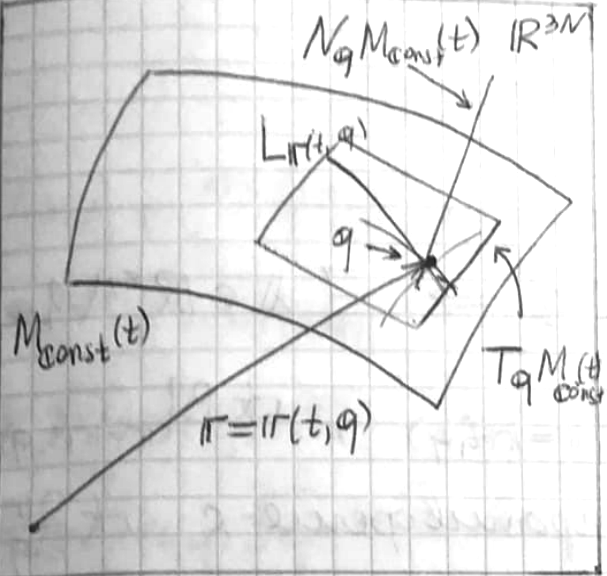
\includegraphics[scale=0.35]{pics/gen_coords}
    \end{center}
    \noindent{\bf Уравнение связей в обобщенных координатах:}
    $$
    \mathcal{A}\bfqd+\bfalpha = 0,\,\,\, \mathcal{A}\in\text{GL}(\mathbb{R}^{k_1},\mathbb{R}^n),\,\,\bfalpha\in\mathbb{R}^{k_1}
    $$
    \begin{lemma} 
    $\rk(\mathcal{A}) = k_1$
    \end{lemma}
    \noindent$\square$ \hyperlink{first_lects.10}{ Доказательство. } $\blacksquare$
    \begin{theorem} (\hyperlink{first_lects.10}{Признак неинтегрируемости связей})\\
    Связь $\mathcal{A}\bfqd+\bfalpha$ -- интегрируемая $\Longleftrightarrow$
    $\bfphi=\bfphi(t,q)=\const$.\\
    $\bfphi(t_1,\bfq_1)\ne\bfphi(t_2,\bfq_2)\,\,\Rightarrow$ систему из $(t_1,\bfq_1)$ в
    $(t_2,\bfq_2)$ нельзя перевести, не нарушая связи.
    \end{theorem}

	\section{Принцип Даламбера – Лагранжа в обобщенных координатах. Уравнения Лагранжа второго рода для голономных систем. Обобщенные силы. Работа сил на перемещении вдоль координатной линии. Случай потенциальных сил. Уравнения Лагранжа со множителями в обобщенных координатах.}
	 \label{3}
	\hyperlink {first_lects.14}{Лекции}\\
	$M_{\const}(t) = \{g = \const\} \subset \mathbb{R}^{3N}$ -- гладкое многообразие, заданное локально.
    \begin{theorem} (\hyperlink{first_lects.14}{Принцип Даламбера-Лагранжа в обобщенных коорд.})\\
    $\bfq=\bfq(t)$ -- движение $(m_i, \bfr_i)_{i=1}^N$ под действием $\bfF$ по
    $M_{\const}(t)$ со связями $\mathcal{A}\bfqd+\bfalpha=\bfzero\,\,$
    $\Longleftrightarrow$\\ $\forall t\in\mathbb{R}:\,$
    $\forall \bfu\in \Ker(\mathcal{A})|_{\bfq=\bfq(t)}:$
    $$
    \begin{cases}
    \left\langle(M\frac{d}{dt}\bfrd-\bfF)^T|_{\bfr=\bfr(r,\bfq),\bfrd=\bfrd(t,\bfq,\bfqd)}\,, \frac{\partial\bfr}{\partial\bfq}|_{\bfq=\bfq(t),\bfqd=\bfqd(t),\bfqdd=\bfqdd(t)}\bfu\right\rangle = 0, \\
    (\mathcal{A}\bfqd+\bfalpha)|_{\bfq=\bfq(t),\bfqd=\bfqd(t)} = \bfzero.\\
    \end{cases}
    $$
    \end{theorem}
    \begin{defn}
    {\it Обобщенная сила} -- $\bfQ^T = \bfF^T|_{\bfr=\bfr(t,\bfq),\bfrd=\bfrd(t,\bfq,\bfqd)}\cdot\frac{\partial\bfr}{\partial\bfq}$.
    \end{defn}
    \begin{example} \hyperlink{first_lects.15}{Работа сил на перемещении вдоль координатной линии (начало страницы)}
    \end{example}
    \noindent{\bf Уравнения Лагранжа 2 рода для голономных систем.}
    \begin{defn} (\hyperlink{first_lects.15}{Уравнения Лагранжа 2 рода})
    $$
    \begin{aligned}
    T = \frac{1}{2}\left\langle M\bfrd,\bfrd\right\rangle = T(\bfrd),\,\,
    \frac{\partial T}{\partial\bfrd} = \bfrd^T M\\
    \frac{d}{dt}(\bfr(t,\bfq))=\frac{\partial\bfr}{\partial t} + \frac{\partial\bfr}{\partial\bfq}\bfqd = \bfrd(t,\bfq,\bfqd)
    \end{aligned}
    $$
    \end{defn}
    \noindent\hyperlink{first_lects.16}{\bf Принцип Даламбера-Лагранжа в обобщенных координатах (другая запись)}
    \begin{example} \hyperlink{first_lects.16}{Уравнения Лагранжа 2 рода для голономных систем}\\
    $k_1 = 0$ -- голономная система.$\forall t\in\mathbb{R}$:\\
    $$\left(\frac{d}{dt}\left(\frac{\partial T}{\partial\bfqd}\bigg|_{\bfrd=\bfrd(t,\bfq,\bfqd)}\right) - \frac{\partial T}{\partial\bfq}\bigg|_{\bfrd=\bfrd(t,\bfq,\bfqd)}\right)\bigg|_{\bfq=\bfq(t),\bfqd=\bfqd(t),\bfqdd=\bfqdd(t)} = \bfQ^T|_{\bfq=\bfq(t),\bfqd=\bfqd(t)}$$
    \end{example}
    \noindent{\bf Случай потенциальных сил.}\\
    \noindent\hyperlink{first_lects.17}{\bf Какой-то пример \note{(видимо важный)}}\\
    {\bf Уравнения Эйлера-Лагранжа:} $$\frac{d}{dt}\frac{\partial L}{\partial\bfqd} - \frac{\partial L}{\partial\bfq} = \bfzero^T$$
    \begin{theorem} (\hyperlink{first_lects.17}{ур-я Лагранжа с множителями в обобщенных коорд.})\\
    $\bfq=\bfq(t)$ -- движение $(m_i, \bfr_i)_{i=1}^N$ под действием $\bfF$ по
    $M_{\const}(t)$ со связями $\mathcal{A}\bfqd+\bfalpha=\bfzero\,\,$
    $\Longleftrightarrow$\\ $\forall t\in\mathbb{R}:\,\exists\,\uplambda=\uplambda(t):$
    $$
    \begin{cases}
    \left(\frac{d}{dt}\frac{\partial T}{\partial\bfqd}\big|_{\bfrd=\bfrd(t,\bfq,\bfqd)} - \frac{\partial T}{\partial\bfq}\big|_{\bfrd=\bfrd(t,\bfq,\bfqd)} - \bfQ^T\right)\bigg|_{\bfq=\bfq(t),\bfqd=\bfqd(t),\bfqdd=\bfqdd(t)} = \uplambda^T\mathcal{A}|_{\bfq=\bfq(t)}\\
    (\mathcal{A}\bfqd+\bfalpha)|_{\bfq=\bfq(t),\bfqd=\bfqd(t)} = \bfzero\\
    \end{cases}
    $$
    \end{theorem}
    \begin{example}\hyperlink{first_lects.17}{Задача Жуковского (внизу страницы)}
    \end{example}
    
    \section{Энергия ускорений. Псевдоскорости. Уравнения Аппеля.}
     \label{4}
   	\hyperlink {first_lects.19}{Лекции}
    \begin{defn} {\it Энергия ускорений:}
    $$
    S = \frac{1}{2}\langle M\bfrdd,\bfrdd\rangle = S(\bfrdd),\,\,\, \frac{\partial S}{\partial\bfrdd} = \bfrdd^T M
    $$
    \end{defn}
    \begin{defn} {\it Псевдоскорости:}
    $$
    \bfomega:\,\, \bfqd = U\bfomega + \bfqd_{\text{чн}},
    $$
    где $\bfqd_{\text{чн}}$ -- частное решение $\mathcal{A}\bfqd+\bfalpha = \bfzero$,\ \ 
    $U = (\bfu_j)_{j=1}^{n-k_1}$.\\ Здесь $\dim\Ker(\mathcal{A}) = n-k_1$ -- {\it число степеней свободы}.
    \end{defn}
    \noindent\hyperlink{first_lects.19}{Подробнее о псевдоскоростях}
    \begin{state} (\hyperlink{first_lects.20}{Уравнение Аппеля})\\
    Сделаем замену $\bfqd = U\bfomega+\bfqd_{\text{чн}} = \bfqd(t,\bfq,\bfomega)$.\\
    $\frac{\partial S}{\partial \dot{\omega}} = \frac{\partial S}{\partial\bfqdd}U$
    \ \ (\hyperlink{first_lects.20}{подробнее об этом в начале страницы})
    $$
    \frac{\partial S}{\partial \dot{\omega}} = \bfQ^T U,\,\,\, \bfqd = U\omega + \bfqd_{\text{чн}}
    $$
    \end{state}
    \noindent\hyperlink{first_lects.20}{\bf Пример.}
    
    \section{Теоремы об изменении импульса, кинетического момента и кинетической энергии для систем со связями и следствия из них.}
    \label{5}
    \hyperlink {first_lects.22}{Лекции}
    \begin{theorem} (\hyperlink{first_lects.22}{Об изменении импульса})\\
    $\bfr=\bfr(t)$ -- движение $(m_i, \bfr_i)_{i=1}^N$ под действием $\bfF$ со
    связями $A\bfrd+\bfa=\bfzero$, и $\forall t\in\mathbb{R}$ связи допускают сдвиг всей
    системы как твердого тела в направлении $\bfe\in\mathbb{R}^3,\, \bfe = \const, \|\bfe\| = 1$. Тогда $\forall t\in\mathbb{R}$:
    $$
    \frac{d}{dt}\langle\bfP,\bfe\rangle|_{\bfrd=\bfrd(t)} = \sum_{i=1}^{N}\langle\bfF_i^{(e)},\bfe\rangle|_{\bfr=\bfr(t),\bfrd=\bfrd(t)}
    $$
    \end{theorem}
    
    \begin{consequence} (\hyperlink{first_lects.23}{Закон сохранения импульса})\\
    Пусть $\sum\limits_{i=1}^N\langle\bfF_i^{(e)},\bfe\rangle = 0$ как $(t,\bfr,\bfrd)$, и
    $\forall (t, \bfr)$ связи допускают сдвиг всей системы как твердого тела в направлении
    $\bfe\in\mathbb{R}^3,\, \bfe = \const, \|\bfe\| = 1$. Тогда $\forall \bfr=\bfr(t) \,\text{-- движения},\,\forall t\in\mathbb{R}$:
    $$
    \langle\bfP,\bfe\rangle|_{\bfrd=\bfrd(t)} = \const.
    $$
    \end{consequence}
    
    \begin{theorem} (\hyperlink{first_lects.24}{Об изменении кинетического момента})\\
    $\bfr=\bfr(t)$ -- движение $(m_i, \bfr_i)_{i=1}^N$ под действием $\bfF$ со
    связями $A\bfrd+\bfa=\bfzero$, и $\forall t\in\mathbb{R}$ связи допускают поворот всей
    системы как твердого тела вокруг оси $O\bfe,\, \bfe\in\mathbb{R}^3,\, \bfe = \const, \|\bfe\| = 1$. Тогда $\forall t\in\mathbb{R}$:
    $$
    \frac{d}{dt}\langle\bfK_0,\bfe\rangle|_{\bfr=\bfr(t),\bfrd=\bfrd(t)} = \langle\bfM_0^{(e)},\bfe\rangle|_{\bfr=\bfr(t),\bfrd=\bfrd(t)}
    $$
    \end{theorem}
    
    \begin{consequence} (\hyperlink{first_lects.24}{Закон сохранения кинетического момента})\\
    Пусть $\langle\bfM_0^{(e)},\bfe\rangle = 0$ как $(t,\bfr,\bfrd)$, и
    $\forall (t, \bfr)$ связи допускают поворот всей системы как твердого тела вокруг оси
    $O\bfe,\, \bfe\in\mathbb{R}^3,\, \bfe = \const, \|\bfe\| = 1$. Тогда $\forall \bfr=\bfr(t) \,\text{-- движения},\,\forall t\in\mathbb{R}$:
    $$
    \langle\bfK_0,\bfe\rangle|_{\bfr=\bfr(t),\bfrd=\bfrd(t)} = \const.
    $$
    \end{consequence}
    
    \begin{theorem} (\hyperlink{first_lects.25}{Об изменении кинетической энергии})\\
    $\bfr=\bfr(t)$ -- движение $(m_i, \bfr_i)_{i=1}^N$ под действием $\bfF$ со
    связями $A\bfrd+\bfa=\bfzero$, и $\forall t\in\mathbb{R}:\,\, \bfrd(t)\in\Ker(A)|_{\bfr=\bfr(t)}$. Тогда:
    $$
    \frac{d}{dt}T|_{\bfrd=\bfrd(t)} = \langle\bfF,\bfrd\rangle|_{\bfr=\bfr(t),\bfrd=\bfrd(t)}
    $$
    \end{theorem}
    
    \begin{consequence} (\hyperlink{first_lects.26}{Закон сохранения энергии})\\
    $\bfr=\bfr(t)$ -- движение $(m_i, \bfr_i)_{i=1}^N$ под действием $\bfF$ со
    связями $A\bfrd+\bfa=\bfzero$, $V=V(\bfr),\, \bfF=-\frac{\partial V^T}{\partial\bfr}$,
    и $\forall t\in\mathbb{R}:\, \bfrd(t)\in\Ker(A)|_{\bfr=\bfr(t)}$. Тогда $\forall t\in\mathbb{R}$:
    $$
    (T+V)|_{\bfr=\bfr(t),\bfrd=\bfrd(t)} = \const
    $$
    \end{consequence}
    
    \section{Эквивалентность принципа Даламбера – Лагранжа и уравнений движения свободного твердого тела.}
     \label{6}
    \hyperlink {first_lects.27}{Лекции} \\
    
    \begin{theorem} (Принцип Даламбера-Лагранжа для свободного тв.тела)
    $\bfr = \bfr(t) $ - движение тв.тела $(m_i, \bfr_i)^N_{i=1}$:\\
    $|\bfr_i - \bfr_j| = c_{ij} > 0$, $i < j = 1, ..., N$ под действием 
    $\bfF \Leftrightarrow \forall t \in R$  $\forall \bfv_c$, $\bfomega \in R^3$ $[|\bfr_i - \bfr_j| |_{ \bfr=\bfr(t)=c_{ij}}, i < j = 1,...,N;$  $<M\ddot{\bfr}(t) - \bfF, \bfv>$ $=0$, 
    где $\bfv = ((\bfv_c + ((\bfomega\times\bfrho_i)^T)^N_{i=1})^T]$
    \end{theorem}    
    
    $\square$
    $\dot{\bfr} = \bfv_c + \bfomega\times\bfrho_i \Rightarrow \bfv = ((\bfv_c + ((\bfomega\times\bfrho_i)^T)^N_{i=1})^T$ - параметрическое задание $KerA$. $\blacksquare$\\
    
    \note{\it Формулировка этой херни, которую я нашел в интернете звучит так:\\ Для системы с идеальными связями в любой момент времени сумма элементарных работ активных сил и даламберовых сил инерции равняется нулю. \\Я бы ей не доверял, но, т.к. сам не понимаю формулировку из лекций, думаю, что ляпнуть можно, если докопаются.}
    
     \begin{theorem} (\hyperlink {first_lects.28}{Следствие})
    $\bfr = \bfr(t)$ - движение твердого тела 
    $(m_i, bfr_i)^N_{i=1}$: $|\bfr_i - \bfr_j| = c_{ij} > 0$, $i<j = 1,...,N$ 
    под действием $\bfF$ $\Leftrightarrow$ $\forall t \in R [|\bfr_i - \bfr_j| |_{\bfr=\bfr(t)=c_{ij}}$,
     $i<j=1,...,N$, $m\ddot{\bfr}_c(t)=\sum\limits^N_{i=1} \bfF^{(e)}_i |_{\bfr=\bfr(t), \dot{\bfr}=\dot{\bfr}(t)}$,
      $\frac{d}{dt}K^{(relative)}_c|_{\bfr=\bfr(t), \dot{\bfr}=\dot{\bfr}(t)} = M^{(e)}_c |_{\bfr=\bfr(t), \dot{\bfr}=\dot{\bfr}(t)}]$
      \end{theorem}
     
    
    \section{Уравнения Лагранжа второго рода. Калибровка. Преобразование уравнений при замене координат.}
     \label{7}
    \hyperlink {first_lects.29}{Лекции} \\
    \begin{defn}(Уравнение Лагранжа второго рода)
		\begin{center}
 			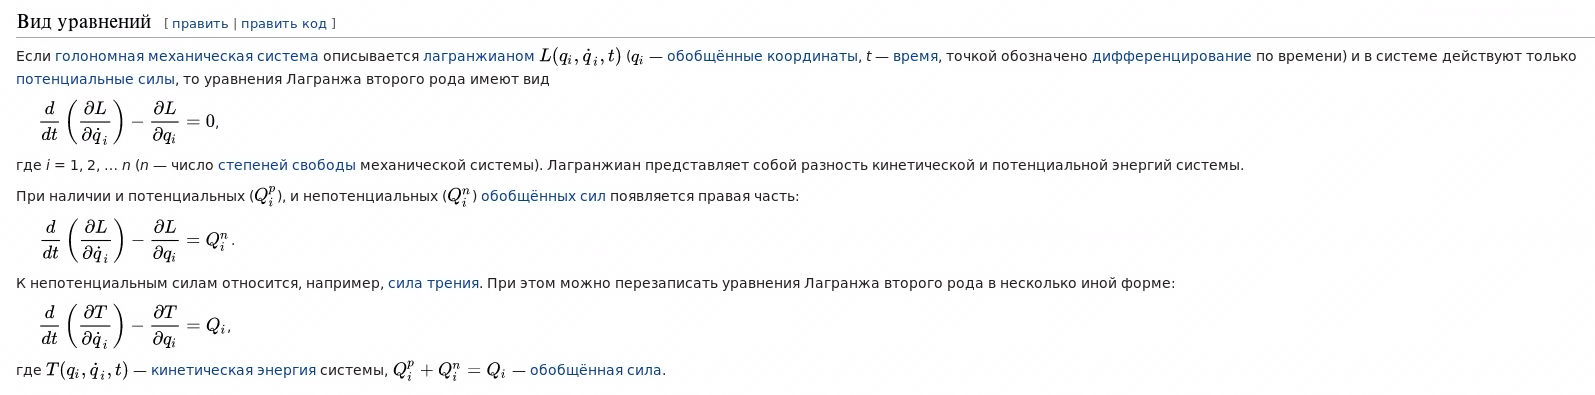
\includegraphics[scale=0.5]{pics/lagranzh}
		\end{center}
	\end{defn}
	
	\noindent\hyperlink {first_lects.29}{Вывод, что они имеют второй порядок см.здесь} \\
	
	\textbf{Калибровка} - $L$ и $\widetilde{L}$ дают одинаковые уравнения Лагранжа второго рода:\\
	$\frac{d}{dt}\frac{\partial L}{\partial \dot{\bfq}} - \frac{\partial L}{\partial \bfq} \Leftrightarrow \frac{d}{dt}\frac{\partial \widetilde{L}}{\partial \dot{\bfq}} - \frac{\partial \widetilde{L}}{\partial \bfq}$\\
	Например, $\widetilde{L} = const L$ или $\widetilde{T} = const  T, \widetilde{Q} = const Q$\\
	\note{\it Я понятия не имею, что происходит, но вроде вики говорит калибровка векторного потенциала — наложение дополнительных условий, позволяющих однозначно вычислить векторный потенциал электромагнитного поля для решения тех или иных физических задач.}\\
	
	\noindent\hyperlink {first_lects.30}{Пример какой-то калибровки} \\
	
	\begin{theorem}(\hyperlink {first_lects.31}{Теорема о преобразовании при замене к-т})\\
	
	\noindent\hyperlink {first_lects.31}{Начальные условия внизу страницы}\\
	
	$\bfx$ - другие локальные к-ты на $M_{const} (t)$\\
	$\frac{d}{dt}[\frac{\partial T}{\partial \dot{\bfx}}|_{\dot{\bfr} = \dot{\bfr}(t, \bfx, \dot{\bfx})}]  -  \frac{\partial T}{\partial \bfx}|_{\dot{\bfr} = \dot{\bfr}(t, \bfx, \dot{\bfx})} = 
	(\frac{d}{dt}[\frac{\partial T}{\partial \dot{\bfq}}|_{\dot{\bfr} = \dot{\bfr}(t, \bfq, \dot{\bfq})}]  -  \frac{\partial T}{\partial \bfq}|_{\dot{\bfr} = \dot{\bfr}(t, \bfq, \dot{\bfq})})|_{\bfq = \bfq(t, \bfx), \dot{\bfq} = \dot{\bfq} (t, \bfx, \dot{\bfx})} \frac{\partial \bfq}{\partial \bfx}$\\
	$\bfX^T =  \bfQ^T |_{\bfq = \bfq(t, \bfx), \dot{\bfq} = \dot{\bfq} (t, \bfx, \dot{\bfx})} \frac{\partial \bfq}{\partial \bfx}$ 
	\end{theorem}
	
	
     
    
    \section{Первые интегралы уравнений Лагранжа для систем с потенциальными силами:    интеграл Якоби, интеграл энергии, циклические интегралы. Поле симметрий. Теорема Нетер.}
     \label{8}
    \hyperlink {lects.1}{Лекции} \\
    \begin{defn}
	Первым интегралом системы $\frac{d}{dt}\frac{\partial L}{\partial \dot{\bfq}} - \frac{\partial L}{\partial \bfq} = 0$ называется функция $f(\dot{\bfq}, \bfq, t)$, которая оказывается константой на любом решении этой системы.   
    \end{defn}
    
    \textbf{Простейшие первые интегралы уравнений Лагранжа}:
    \begin{itemize}
    \item[1] $\bfq = (\overline{\bfq}^T, \widetilde{\bfq}^T)^T$, $\frac{\partial L}{\partial \overline{\bfq}} \Leftrightarrow L=(t, \widetilde{\bfq}, \dot{\bfq}) \Rightarrow \frac{\partial L}{\partial \dot{\overline{\bfq}}}$ - циклические интегралы
    \item[2] Если $\frac{\partial L}{\partial t}$, то $H(\dot{\bfq}, \bfq, t) = \frac{\partial L^T}{\partial \dot{\bfq}} \dot{\bfq} - L = const$
    \item \hyperlink {lects.1}{Подробности} 
    \end{itemize}
    
    \begin{theorem}(Замечание)\\
   		Для уравнений механики $L = T_2+T_1+T_0-V=L_2+L_1+L_0$
    \end{theorem}
    \begin{defn} (\hyperlink {lects.1}{Интеграл Якоби})\\
    	$H=T_2-T_0+V=L_2-L_0=const$ 
    \end{defn}
    \begin{defn} (Интеграл энергии)\\
    	Это интеграл Якоби при $T \equiv T_2$: $H=T+V=h=const$\\
    \end{defn}
    
    \noindent\hyperlink {lects.1}{Примеры в конце страницы}\\
    
    \begin{defn}
    	Вектор $\bfv(\bfq) \in R^n$ называется полем симметрий системы с функцией Лагранжа $L=L(\dot{\bfq}, \bfq, t)$, если на любом решении $\bfq(\tau), \dot{\bfq}(\tau)$ системы $\{\bfq' = \bfv(\bfq), (\dot{\bfq})'=\frac{\partial \bfv}{\partial \bfq} \dot{\bfq}\}$ для любого $t$ :\\
    	\begin{center}
    	$\frac{d}{d\tau} L (\dot{\bfq}(\tau), \bfq(\tau), t) \equiv 0$
    	\end{center}
    \end{defn}
    
    \begin{theorem}(\hyperlink {lects.2}{Нётер})\\
    Если $\bfv(\bfq)$ поле симметрий системы с функций Лагранжа $L(\dot{\bfq}, \bfq, t)$, то уравнения Лагранжа имеют первый интеграл $I=\frac{\partial L^T}{\partial \dot{\bfq}} \bfv(\bfq) = const$
    \end{theorem}
    
    
    
    \section{Понижение порядка уравнений Лагранжа по Раусу. Функция Рауса. Приведенный потенциал. Уравнения Рауса.}
     \label{9}
    \hyperlink {lects.3}{Лекции} \\
    
    \begin{defn} 
    { \it Понижение порядка системы уравнений Лагранжа по Раусу} \---
    	использование циклических интегралов\\
    \end{defn}
    
    \begin{defn} 
    { \it Функцией Рауса} системы с функцией Лагранжа $L=L(\dot{\bfq}, \widetilde{\bfq}, t)$ называется $R(\dot{\widetilde{\bfq}}, \widetilde{\bfq}, t, \bfc) = (L - \frac{\partial L^T}{\partial \dot{\overline{\bfq}}} \dot{\overline{\bfq}})_{*} - L|_{*} - \bfc^T\overline{\phi}(\dot{\widetilde{\bfq}}, \widetilde{\bfq}, t, \bfc)$, где (*) означает подстановку $\dot{\overline{\bfq}} = \overline{\phi} (\dot{\widetilde{\bfq}}, \widetilde{\bfq}, t, \bfc)$
    \end{defn}
    
    \begin{theorem}(\hyperlink {lects.4}{Теорема Рауса})\\
    Если $\overline{\bfq}$ - циклические координаты системы с функцией Лагранжа $L$ и $det \frac{\partial^2 L}{\partial \dot{\overline{\bfq}}^2} \neq 0$, то уравнения 
    \begin{center}
    $\frac{d}{dt} (\frac{\partial L}{\partial \dot{\bfq}}) - \frac{\partial L}{\partial \bfq} = 0$   (I)
    \end{center}
    эквивалентны системе уравнений
    \begin{equation*}
 		\begin{cases}
  			 \frac{d}{dt}(\frac{\partial R}{\partial \dot{\widetilde{\bfq}}}) - \frac{\partial R}{\partial \bfq} = 0,   (II)
   				\\
  			 \dot{\widetilde{\bfq}} = \overline{\phi} (\dot{\widetilde{\bfq}}, \widetilde{\bfq}, t, \bfc), \dot{\bfc} = 0  (III)
  				
		\end{cases}
	\end{equation*}, где $R(\dot{\widetilde{\bfq}}, \widetilde{\bfq}, t, \bfc)$ \--- функция Рауса системы с функцией Лагранжа $L$.
    \end{theorem}
    
    \begin{defn} 
    (II) \--- { \it уравнения Рауса}\\
    (II, III) \--- {\it приведенная система}\\
    Переход от (I)  к (II,III) \--- {\it понижение порядка по Раусу (игнорирование циклических к-т)}
    \end{defn}
    
    В задачах механики часто оказывается $R= R_2+R_1+R_0$, где смысл индексов тот же, что и в типичной ф-ии Лагранжа, только по отношению к $\dot{\widetilde{\bfq}}$
    
      \begin{defn} 
    Функция $V_\bfc = -R_0$ \--- называется {\it приведенным потенциалом}
    \end{defn}
    
    \noindent\hyperlink {lects.5}{Пример}\\
    
    
    \section{Задача Лагранжа о вращении тяжелого твердого тела вокруг неподвижной точки. Типичное движение оси динамической симметрии. Псевдорегулярная и регулярная прецессии. Способы реализации движений этих типов с заданным углом нутации.}
     \label{10}
    \hyperlink {lects.6}{Лекции} \\
    \begin{defn} 
    	{\it Задача Лагранжа} о движении твердого тела с неподвижной точкой \--- это пример использования понижения порядка уравнений Лагранжу по Раусу
    \end{defn}
     \noindent\hyperlink {lects.6}{Разбор задачи}\\
      \noindent\hyperlink {lects.7}{Типичное движение оси динамической симметрии со слов "Известно, что"}\\
    
    \begin{defn} 
    	{\it Псевдорегулярная процессия} \--- движение конца вектора $e_3$ будет происходит между сколь угодно близкими параллелями на единичной сфере.
    \end{defn}
    \begin{defn} 
    	{\it Регулярная процессия} \--- похоже на регулярную, но нет точек остановки конца $e_3$. $\eta = \eta_0=const$, $\dot{\phi}=const$, $\dot{\psi} = const$
    \end{defn}
    
     \noindent\hyperlink {lects.7}{Способы реализации движений этих типов с заданным углом нутации -  внизу со слов "Докажем, что..."}\\
    
    \section{Равновесия системы уравнений Лагранжа. Соответствующие движения механической системы. Уравнения равновесия. Устойчивость равновесий по Ляпунову. Теорема Лагранжа – Дирихле о достаточном условии устойчивости равновесия.}
     \label{11}
    \hyperlink {lects.10}{Лекции} \\
    	\begin{defn}
    		\textbf{Равновесие системы уравнений Лагранжа} с заданной функцией Лагранжа в некоторых координатах $\bfq$ - это частное решение 
    		$$
    			\bfq = \bfq_* = const
    		$$
    	\end{defn}
    
    	Для соответствующей механической системы с конфигурационным многообразием $M$ это либо состояние покоя $\bfr = \bfr(\bfq_*)$ (когда многообразие не зависит от $t$, т.е. $\bfr=\bfr(\bfq)$), либо специальное движение $\bfr = \bfr_*(t) = \bfr(\bfq_*,t)$, которое можно интерпретировать, как равновесие на подвижном многообразии с уравнением $\bfr=\bfr(\bfq,t)$ - \textit{относительное равновесие}.
    	
    	\textbf{Уравнение равновесия} \\
    	Рассмотрим систему с конфигурационным многообразием $M:\bfr = \bfr(\bfq)$ в координатах $\bfq \in \mathbb{R}^n$ и потенциальными силами с потенциальной энергией $V(\bfq)$, не зависящей от времени. Для нее 
    	$$
    		L = T - V = \frac{1}{2}\dot{\bfq}^T A(\bfq) \dot{\bfq} - V(\bfq)
    	$$
    	и $\bfq_* = const$ - равновесие соответствующей системы уравнений Лагранжа тогда и только тогда, когда
    	$$
    		\left. \frac{\partial V}{\partial \bfq} \right|_{\bfq_*} = 0
    	$$
    	\hyperlink {lects.10}{Д-во: (3)} \\
    	
    	\textbf{\hyperlink {lects.10}{Устойчивость равновесий по Ляпунову (5)}} \\
    	В фазовом пространстве $(\bfq,\dot{\bfq})$ для $a>0$ обозначим $C_a$ множество $|\dot{\bfq}| <a, \ |\bfq-\bfq_*| < a$, где под $|\textbf{f}|$ понимается $|f_i| < a, \ i = 1,2,...,n$.
    	\begin{defn}
    		Равновесие системы с функцией Лагранжа $L = \frac{1}{2}\dot{\bfq}^T A(\bfq) \dot{\bfq} - V(\bfq)$ называется \textbf{устойчивым по Ляпунову}, если $\forall \ \varepsilon > 0 \ \exists \ \delta > 0 : \ \forall \ \bfq(t)$ - решения системы $\frac{d}{dt}\left( \frac{\partial L}{\partial \dot{\bfq}} \right) - \frac{\partial L}{\bfq} = 0$ с начальным условием $(\bfq_0, \dot{\bfq}_0)\in C_{\delta}$ при $t = 0$ для всех $t > 0$ верно $(\bfq(t), \dot{\bfq}(t)) \in C_{\varepsilon}$.
    	\end{defn}  
    
    	\begin{theorem}
    		(\textbf{Лагранжа-Дирихле о достаточном условии равновесия}\hyperlink {lects.10}{(конец страницы)}) \\
    		Если $\bfq = \bfq_*$ - точка строго локального минимума функции $V(\bfq)$, то равновесие $\bfq = \bfq_*$ системы уравнений Лагранжа с функцией Лагранжа $L = \frac{1}{2}\dot{\bfq}^T A(\bfq) \dot{\bfq} - V(\bfq)$ устойчиво по Ляпунову.
    	\end{theorem}
    \section{Линеаризация уравнений Лагранжа в окрестности состояния равновесия. Существование нормальных координат. Линеаризованные уравнения в нормальных координатах, их интегрирование. Уравнение для собственных чисел. Независимость собственных чисел от выбора координат. Собственные векторы. Выражение матрицы преобразования к нормальным координатам через компоненты собственных векторов.}
     \label{12}
    \hyperlink {lects.11}{Лекции (конец страницы)} \\
    
    \textbf{Линеаризация уравнений Лагранжа около состояния равновесия} \\
    Берем функция Лагранжа
    $$
   		L = T - V = \frac{1}{2}\dot{\bfq}^T A(\bfq) \dot{\bfq} - V(\bfq)
    $$
    и подставляем в уравнение Лагранжа
    $$
    	\frac{d}{dt}\left( \frac{\partial L}{\partial \dot{\bfq}} \right) - \frac{\partial L}{\bfq} = 0
    $$
    получаем 
    $$
    	A \overset{..}{\bfq} + \frac{d}{dt}\left( A \right) \dot{\bfq} - \frac{\partial}{\partial \bfq} \left(\frac{1}{2} \dot{\bfq}^T A \dot{\bfq} \right) + \frac{\partial V}{\partial \bfq} = 0 \ \ \ \hyperlink {lects.10}{(4)}
    $$
    и раскладываем это в ряд Тейлора до первой степени вокруг точки $(0,0,\bfq_*)$ (мы как бы в пространстве с координатами $(\overset{..}{\bfq}, \dot{\bfq}, \bfq)$), где $\bfq_*$ - равновесие. После отбрасывания хвоста со степенями выше первой останется линейный кусок:
    $$
    	A_* \overset{..}{\bfq} + \Pi_* (\bfq - \bfq_*) = 0
    $$
    где $A_* = A(\bfq_*), \ \Pi_* = \left. \frac{\partial^2 V}{\partial \bfq^2} \right|_{\bfq_*}$. Это и есть \textbf{\hyperlink{lects.12}{линеаризованное уравнение (7)}}.
    
    \bigskip  
    \textbf{\hyperlink{lects.12}{Нормальные координаты (12)}}
    \begin{defn}
    	Рассмотрим такое линейное преобразование координат $\bfq - \bfq_* = C\bfx$ и $\dot{\bfq} = C\bfx$, при котором линеаризованное уравнение примет вид
    	$$
    		\overset{..}{\bfx} + \Lambda \bfx = 0
    	$$ 
    	т.е. такое преобразование, которое две квадратичные формы $A_*$ и $\Pi_*$ приводит соответственно в лиду $E$ - единичная и $\Lambda = diag\{\lambda_i\}, \ i = 1,...,n$. Такие координаты $\bfx$ называются \textbf{нормальными}.
    \end{defn}  
	Их \textbf{\hyperlink{lects.12}{существование (11-12)}} следует непосредственно из приведения обеих квадратичных форм к нужному виду.
	
	\begin{defn}
		Числа $\lambda_i$ (диагональ матрицы $\Lambda$ из определения выше) называются собственными числами пары квадратичных форм с матрицами $A_*$ и $\Pi_*$.
	\end{defn}  

	\begin{state}
		 \hyperlink {lects.12}{(13)} Собственные числа - это корни уравнения $$det (\lambda A_* - \Pi_*) = 0$$
	\end{state}

	\begin{state}
		Собственные числа не зависят от выбора координат $\bfq$. \hyperlink {lects.12}{(конец страницы)}
	\end{state} 

	\begin{defn}
		Вектор $\textbf{c} \in \mathbb{R}^n$ - \textbf{собственный вектор}, отвечающий собственному значению $\lambda$, если $$(\lambda A_* - \Pi_*)\textbf{c} = 0$$
	\end{defn} 

	\begin{state}
		Столбец $\textbf{c}_i$ матрицы  перехода к нормальным координатам $C$ - собственный вектор, соответствующий собственному значению $\lambda_i$. \hyperlink {lects.13}{(утверждение)}
	\end{state}  

	\bigskip
	\textbf{\hyperlink {lects.13}{Решения $\bfx_i$ независимых уравнений в нормальных координатах в зависимости от знака $\lambda_i$ (после (15))}}
	
	\bigskip
	\textbf{\hyperlink {lects.13}{Пример. Одинаковые точки, связанные пружиной на одинаковых окружностях (конец страницы)}}

	
    
    \section{Преобразование уравнений Лагранжа в уравнения Гамильтона. Обобщенные импульсы. Явный вид функции Гамильтона для уравнений механики.}
     \label{13}
     \hyperlink {lects.16}{Лекции} \\
    
        
    \section{Первые интегралы уравнений Гамильтона. Скобки Пуассона в канонических координатах. Свойства скобок Пуассона, тождество Якоби. Простейшие первые интегралы в случаях независимости функции Гамильтона от времени, наличия циклических координат, отделения переменных.}
     \label{14}
    \hyperlink {lects.18}{Лекции} \\
    
    \section{Аналог теоремы Нетер для уравнений Гамильтона. Теорема о скобке Пуассона двух первых интегралов. Скобки Пуассона компонент кинетического момента свободной точки.}
     \label{15}
    \hyperlink {lects.18}{Лекции} \\
    
 \section{Канонические преобразования. Определение, его переформулировка в терминах скобок Пуассона, интерпретация в случае системы с одной степенью свободы. Примеры: тождественное, обратное к каноническому, ортогональное преобразование фазовой плоскости, полярные канонические координаты, каноническая перестановка, каноническое изменение масштабов на координатных осях.}
     \label{16}
    \hyperlink {lects.23}{Лекции} \\
    Произвольная замена неизвестных ведет к разрушает какноническую форму.
    Существует класс преобразований координат в фазовом пространстве, которые сохраняют каноническую форму уравнений Гамильтона. Рассмотрим подмножество - унивалентные канонические преобразования. Называем их каноническими.\\
Воспользуемся обозначением $z = 
\left (
\begin{matrix}
\mathbf{q} \\ \mathbf{p}
\end{matrix}
\right )
$ для исходных канон. уравнений.\\
$
\left \lbrace
\begin{matrix}
\dot{\mathbf{q}} &= \frac{\partial H}{\partial \mathbf{p}}\\
\dot{\mathbf{p}} &= -\frac{\partial H}{\partial \mathbf{q}}
\end{matrix}
\right.
$, $H(\mathbf{p}, \mathbf{q}, t) = H(\mathbf{z}, t)$, запишем через $\dot{\mathbf z} = I \frac{\partial H}{\partial \mathbf z}$, где $I = 
\left (
\begin{matrix}
0&1\\-1&0
\end{matrix}
\right )$\\
Пусть $\mathbf{\zeta} = 
\left (
\begin{matrix}
\mathbf{Q}\\\mathbf{P}
\end{matrix}
\right )
$ - новые координаты, $
\left \lbrace
\begin{matrix}
\mathbf{Q} &= \mathbf{Q}(\mathbf{q}, \mathbf{p}, t)\\
\mathbf{P} &= \mathbf{P}(\mathbf{q}, \mathbf{p}, t) 
\end{matrix}
\right .
, 
\left .
\begin{matrix}
\mathbf{\zeta} = \mathbf{\zeta}(\mathbf{z}, t)\\
J = \frac{\partial \mathbf{\zeta}}{\partial \mathbf{z}} , \det J \neq 0
\end{matrix}
\right .
(3)$\\
\begin{defn} Преобр. (3) наз. каноническим, если $\mathcal{P} = JIJ^\top \equiv I$ \end{defn}
\begin{state} Матрица $\mathcal{P}$ состоит из скобок Пуассона функций, задающих преобразование.\end{state} 
$J = 
\left (
\begin{matrix}
\mathbf{Q}_\mathbf{q}&\mathbf{Q}_\mathbf{p}\\
\mathbf{P}_\mathbf{q}&\mathbf{P}_\mathbf{p}
\end{matrix}
\right )
,\mathbf{Q}_\mathbf{q} = \frac{\partial \mathbf{Q}}{\partial \mathbf{q}},\dots$, то $\mathcal{P} =
\left (
\begin{matrix}
\mathbf{Q}_\mathbf{q}\mathbf{Q}_\mathbf{p}^\top - \mathbf{Q}_\mathbf{p}\mathbf{Q}_\mathbf{q}^\top
&
\mathbf{Q}_\mathbf{q}\mathbf{P}_\mathbf{p}^\top - \mathbf{Q}_\mathbf{p}\mathbf{P}_\mathbf{q}^\top\\
\mathbf{P}_\mathbf{q}\mathbf{Q}_\mathbf{p}^\top - \mathbf{P}_\mathbf{p}\mathbf{Q}_\mathbf{q}^\top
&
\mathbf{P}_\mathbf{q}\mathbf{P}_\mathbf{p}^\top - \mathbf{P}_\mathbf{p}\mathbf{P}_\mathbf{p}^\top\\
\end{matrix}
\right )
$\\
$(\mathbf{Q}_\mathbf{q}\mathbf{Q}_\mathbf{p}^\top - \mathbf{Q}_\mathbf{p}\mathbf{Q}_\mathbf{q}^\top)_{ij}= \sum_k(\frac{\partial Q_i}{\partial q_k}*\frac{\partial Q_j}{\partial p_k} - \frac{\partial Q_i}{\partial p_k}*\frac{\partial Q_j}{\partial q_k}) \Rightarrow \mathcal{P} =
\left (
\begin{matrix}
\{Q_i,Q_j\}&\{Q_i,P_j\}\\
\{P_i,Q_j\}&\{P_i,P_j\}
\end{matrix}
\right )
$\\
Критерий каноничности преобразования (3) в виде :
$$
\{Q_i,Q_j\} \equiv 0, \{P_i,P_j\} \equiv 0, \{P_i,P_j\} \equiv \delta_{ij}, i,j = 1,\dots,n; \delta_{ij} = 
\left \{
\begin{matrix}
0, i\neq j\\1, i = j
\end{matrix}
\right .(6)
$$
\emph{Следствие.}В случае $n = 1$ от уловий (6) остаётся только $\{Q,P\} \equiv 1$ или $\frac{\partial Q}{\partial q}*\frac{\partial P}{\partial p} - \frac{\partial Q}{\partial p}*\frac{\partial P}{\partial q} \equiv 1$, что означает $\det J \equiv 1$\\
\hyperlink {lects.24}{Примеры канонческих преобразований} \\

 \section{Критерии каноничности преобразования.}
     \label{17}
    \hyperlink {lects.25}{Лекции}
\begin{state}
Если каноническое преобразование не зависит от времени, то уранение Гамильтона в новых координатах имеют каноническую форму с той же функцией Гамильтона, только выраженной через новые координаты. \hyperlink {lects.25}{Доказательство} второй абзац
\end{state}
\emph{Замечание} Из (3)(в Док-ве) следует возможность простого обобщения определения канонического преобразования: $JIJ^\top \equiv CI$, где C = const. С называется валентностью канон. преобр. (Считаем C = 1)\\
Сами критерии :\\
Пусть формулы преобразования имеют вид :\\ $\mathbf{\zeta}$ - координаты, $\mathbf{\zeta_0}$ - функции, $\mathbf{\zeta} = \mathbf{\zeta_0}(\mathbf{z},t),
\left \lbrace
\begin{matrix}
\mathbf{Q} &= \mathbf{Q_0}(\mathbf{q}, \mathbf{p}, t)\\
\mathbf{P} &= \mathbf{P_0}(\mathbf{q}, \mathbf{p}, t) 
\end{matrix}
\right .
, 
J = \frac{\partial \mathbf{\zeta_0}}{\partial \mathbf{z}} (4)$\\
\begin{enumerate}
\item {Преобразование (4) каноническое тогда и только тогда, \\когда $J^\top IJ \equiv I$. \hyperlink {lects.25}{Док-во в конце страницы}}
\item {Преобразование (4) каноническое тогда и только тогда, когда тождественно равна нулю 2-форма $\sum dp_i \wedge dq_i - \sum \delta P_{\ddot a} \wedge \delta Q_{\ddot a} \equiv 0$ или $d\mathbf{p} \wedge d \mathbf{q} - \delta \mathbf{P}_0^\top\wedge \delta \mathbf{Q}_0 \equiv 0$ (7).\\
Можно выразить $\delta \mathbf{P}_0^\top\wedge \delta \mathbf{Q}_0 \equiv -\frac{1}{2}\delta \mathbf{\zeta_0}^\top \wedge \delta\mathbf{\zeta_0}$. \hyperlink {lects.26}{Док-во в начале}}\\
\emph{Лемма Пуанкаре} Для 1-формы $\omega$ тождество $\delta \omega \equiv 0$ верно тогда и только тогда, когда существует такая функция $f(\mathbf{z}, t)$, что $\omega \equiv \delta f$.
\item -//-, если существует такая функция $\Pi(\mathbf{z}, t)$, что\\ $\mathbf{p} \wedge d \mathbf{q} - \mathbf{P}_0^\top\wedge \delta \mathbf{Q}_0 \equiv \delta \Pi(\mathbf{z}, t)$\hyperlink {lects.27}{Док-во в начале}
\end{enumerate}
    \section{Преобразование уравнений Гамильтона при канонических преобразованиях.}
     \label{18}
    \hyperlink {lects.27}{Лекции} \\
\emph{Лемма} Уравнение Гамильтона $\left.
\begin{matrix}
\dot{\mathbf{q}} &= \frac{\partial H}{\partial \mathbf{p}}\\
\dot{\mathbf{p}} &= -\frac{\partial H}{\partial \mathbf{q}}
\end{matrix}
\right.
$- это уравнение Лагранжа в координатах $z = 
\left (
\begin{matrix}
\mathbf{q} \\ \mathbf{p}
\end{matrix}
\right )
$ с функцией Лагранжа $\mathcal{L}(\dot{\mathbf{z}},\mathbf{z}, t) = \mathbf{p}^\top \dot{\mathbf{q}} - H(\mathbf{q},\mathbf{p}, t).(9)$ \hyperlink {lects.27}{Док-во в конце}

    \section{Производящие функции канонических преобразований (свободного и стандартного). Выражение новой функции Гамильтона через производящие функции в этих случаях. Производящие функции для преобразований: тождественного, перехода к полярным каноническим координатам, канонической перестановки, канонического изменения масштабов на координатных осях.}
     \label{19}
    \hyperlink {lects.28}{Лекции (низ страницы)} \\
Рассмотрим только два случая :\\
Свободное каноническое преобразование : пусть в формулах (4) канонического преобразования $\det (\frac{\partial \mathbf{Q_0}}{\partial \mathbf{p}}) \neq 0$.     
\hyperlink {lects.29}{Формулы и преобразования в начале} \\
Стандартное каноническое преобразование : пусть в формулах (4) канонического преобразования $\det (\frac{\partial \mathbf{ P_0}}{\partial \mathbf{p}}) \neq 0$.     
\hyperlink {lects.29}{Ф-лы и преобр-ния в конце} \\
\textit{Выражение новой ф-ии Гамильтона через производящую ф-ию}\\
Используем функцию Лагранжа(9). Переходим к координатам $(\mathbf{q},\mathbf{Q})$.
\hyperlink {lects.30}{Все преобразования на этой странице} \\
\textit{Замечания о канонических преобразованиях с производящей ф-ей}\\
1) Любое каноническое преобразование имеет производящую функцию.\\
\hyperlink {lects.30}{Все примеры в начале страницы} \\
2) Если $\bar{S}(\mathbf{q},\mathbf{Q}, t)$ - функция от $\mathbf{q} \in \mathbb{R}^n, \mathbf{Q} \in \mathbb{R}^n, t; \det \frac{\partial^2 \bar{S}}{\partial \mathbf{Q} \partial \mathbf{q}} \neq 0$, то формулы $\left \{
\begin{matrix}
\mathbf{p}&= \frac{\partial \bar S}{\partial \mathbf{q}}\\
\mathbf{P} &= -\frac{\partial \bar S}{\partial \mathbf{Q}}
\end{matrix}
\right .$ задают каноническое преобразование $\left (
\begin{matrix}
\mathbf{q}\\ \mathbf{p}
\end{matrix}
\right ) \rightarrow \left (
\begin{matrix}
\mathbf{Q}\\ \mathbf{P}
\end{matrix}
\right )$\\
Аналогично, если $\tilde{S}(\mathbf{q},\mathbf{P}, t)$ такова, что $\det \frac{\partial^2 \tilde{S}}{\partial \mathbf{P} \partial \mathbf{q}} \neq 0$, то формулы $\left \{
\begin{matrix}
\mathbf{p}&= \frac{\partial \tilde S}{\partial \mathbf{q}}\\
\mathbf{Q} &= \frac{\partial \tilde S}{\partial \mathbf{P}}
\end{matrix}
\right .$ задают каноническое преобразование $\left (
\begin{matrix}
\mathbf{q}\\ \mathbf{p}
\end{matrix}
\right ) \rightarrow \left (
\begin{matrix}
\mathbf{Q}\\ \mathbf{P}
\end{matrix}
\right )$ \hyperlink {lects.31}{Док-ва в конце} \\
 \section{Уравнения для производящих функций целенаправленных канонических преобразований. Уравнение Гамильтона – Якоби, его полный интеграл. Теорема Якоби. Нахождение полного интеграла в случаях независимости функции Гамильтона от времени, наличия циклических координат, отделения переменных.}
     \label{20}
    \hyperlink {lects.32}{Лекции} \\
    Пусть требуется найти каноническое преобразование $\left (
\begin{matrix}
\mathbf{q}\\ \mathbf{p}
\end{matrix}
\right ) \rightarrow \left (
\begin{matrix}
\mathbf{Q}\\ \mathbf{P}
\end{matrix}
\right )$, что функция, имеющая в координатах $(\mathbf{q}, \mathbf{p})$ формулу $f(\mathbf{q}, \mathbf{p}, t)$, приобретает в коорлинатах $(\mathbf{Q}, \mathbf{P})$ формулу $g(\mathbf{Q}, \mathbf{P}, t)$. Ищем производящую функцию вида $\tilde{S}(\mathbf{q},\mathbf{P}, t)$, $\det \frac{\partial^2 \tilde{S}}{\partial \mathbf{q} \partial \mathbf{P}} \neq 0$, как решение дифференциального уравнения в частных производных : $f(\mathbf{q}, \frac{\partial \tilde{S}}{\partial \mathbf{q}}, t) = g(\frac{\partial \tilde{S}}{\partial \mathbf{P}}, \mathbf{P}, t).$\\
Если $S_0(\mathbf{q},\mathbf{P}, t)$ - одна из таких функций, то формулы $\left \{
\begin{matrix}
\mathbf{p}&= \frac{\partial \tilde S_0}{\partial \mathbf{q}}\\
\mathbf{Q} &= \frac{\partial \tilde S_0}{\partial \mathbf{P}}
\end{matrix}
\right .$ задают каноническое преобразование $\left \lbrace
\begin{matrix}
\mathbf{Q} &= \mathbf{Q_0}(\mathbf{q}, \mathbf{p}, t)\\
\mathbf{P} &= \mathbf{P_0}(\mathbf{q}, \mathbf{p}, t) 
\end{matrix}
\right .$, причем тождество $f(\mathbf{q}, \frac{\partial \tilde{S_0}}{\partial \mathbf{q}}, t) = g(\frac{\partial \tilde{S_0}}{\partial \mathbf{P}}, \mathbf{P}, t).$ в координатах $(\mathbf{q}, \mathbf{p})$ примет вид \\
$f(\mathbf{q}, \mathbf{p}, t) \equiv g( \mathbf{Q_0}(\mathbf{q}, \mathbf{p}, t),  \mathbf{P_0}(\mathbf{q}, \mathbf{p}, t), t).$\\
Для функции $\bar{S}(\mathbf{q},\mathbf{P}, t)$, $\det \frac{\partial^2 \bar{S}}{\partial \mathbf{q} \partial \mathbf{P}} \neq 0$, достаточно найти такое решение уравнения $f(\mathbf{q}, \frac{\partial \bar{S}}{\partial \mathbf{q}}, t) = g( \mathbf{Q},-\frac{\partial \bar{S}}{\partial \mathbf{Q}}, t).$\\
\textit{Преобразование функции Гамильтона}\\
Если каноническое преобразование $\left (
\begin{matrix}
\mathbf{q}\\ \mathbf{p}
\end{matrix}
\right ) \rightarrow \left (
\begin{matrix}
\mathbf{Q}\\ \mathbf{P}
\end{matrix}
\right )$ не зависит от времени, то новая ф-ия Гамильтона $\mathcal{H}(\mathbf{Q}, \mathbf{P}, t)$ получается из старой$H(\mathbf{q}, \mathbf{p}, t)$ подстановкой формул замены. Для достижения цели $H(\mathbf{q}, \mathbf{p}, t)\rightarrow\mathcal{H}(\mathbf{Q}, \mathbf{P}, t)$ достаточно найти не зависящее от времени решение уравнения \\
$H(\mathbf{q}, \frac{\partial S}{\partial \mathbf{q}}, t) = \mathcal{H}(\frac{\partial S}{\partial \mathbf{P}}, \mathbf{P}, t)$, удовлетворяюее условию невырожденности\\
$\det \frac{\partial^2 S}{\partial \mathbf{q} \partial \mathbf{P}} \neq 0$ и использовать формулы $\mathbf{p} = \frac{\partial S}{\partial \mathbf{q}}$,$
\mathbf{Q} = \frac{\partial S}{\partial \mathbf{P}}.$\\
При использовании преобразований, зависящих от времени и имеющих производящую функцию $S(\mathbf{q},\mathbf{P}, t)$, новая ф-ия Гамильтона $\mathcal{H}(\mathbf{Q}, \mathbf{P}, t)$ получаетс из старой $H(\mathbf{q}, \mathbf{p}, t)$ по формуле\\
 $\mathcal{H}(\mathbf{Q}, \mathbf{P}, t) = (H(\mathbf{q},\frac{\partial S}{\partial \mathbf{q}}, t) + \frac{\partial S}{\partial t})|_{(\mathbf{Q}, \mathbf{P})} (4)$\\
Поэтому для достижения нужной цели $H(\mathbf{q}, \mathbf{p}, t)\rightarrow\mathcal{H}(\mathbf{Q}, \mathbf{P}, t)$, достаточно найти решение $S(\mathbf{q},\mathbf{P}, t)$ уравнения\\
$H(\mathbf{q},\frac{\partial S}{\partial \mathbf{q}}, t) + \frac{\partial S}{\partial t} = \mathcal{H}(\frac{\partial S}{\partial \mathbf{P}}, \mathbf{P}, t)$, со свойствомом $\det \frac{\partial^2 S}{\partial \mathbf{q} \partial \mathbf{P}} \neq 0$\\
\textit{Метод Якоби интегрирования уравнений Гамильтона}\\
Рассмотрим уравнение $\left \lbrace
\begin{matrix}
\dot{\mathbf{q}} &= \frac{\partial H}{\partial \mathbf{p}}\\
\dot{\mathbf{p}} &= -\frac{\partial H}{\partial \mathbf{q}}
\end{matrix}
\right.(5)
$, $H = H(\mathbf{p}, \mathbf{q}, t)$, $\mathbf{q},\mathbf{p} \in \mathbb{R}^n.$\\
Соответствующим уравнением Гамильтона-Якоби называется уравнение в частных производных $H(\mathbf{q},\frac{\partial S}{\partial \mathbf{q}}, t) + \frac{\partial S}{\partial t} = 0$	(6)\\
Семейство решений $S(\mathbf{q},\mathbf{P}, t)$, зависящее от $n$ параметров $\mathbf{P} \in \mathbb{R}^n$, удовлетворяющее условию нвырожденности $\det \frac{\partial^2 S}{\partial \mathbf{q} \partial \mathbf{P}} \neq 0 (7)$ называется его полным интегралом.
\begin{theorem}Якоби. Если $S(\mathbf{q},\mathbf{P}, t)$ - полный интеграл уравнения Гамильтона-Якоби системы (5), то общее решение системы (5) получается из уравнения $\left \lbrace \begin{matrix}
\mathbf{P} &= \frac{\partial S(\mathbf{q},\mathbf{P_0}, t)}{\partial \mathbf{q}}\\
\mathbf{Q_0} &= \frac{\partial S(\mathbf{q},\mathbf{P_0}, t)}{\partial \mathbf{P_0}}
\end{matrix}
\right . (8)
$, где $\mathbf{Q_0} \in \mathbb{R}^n, \mathbf{P_0} \in \mathbb{R}^n$ - произвольные постоянные. \hyperlink {lects.33}{Доказательство в конце страницы}
\end{theorem}
\textit{Замечание.} Эта теорема - частный случай более общей теоремы из теории уравнений в частных производных первого порядка. В терминах этой общей теории систеа (5) - это уравнения характеристик для уравнения (6).\\
Метод Якоби - это описанный алгоритм получения решения (11)(из Док-ва) в неявном виде (8). Главная его проблема - нахождение полного интеграла уравнения (6). Приведем список простейших случаев, когда решение этой проблемы можно облегчить.\\
\hyperlink {lects.34}{С середины страницы идёт 4 пункта} \\
\hyperlink {lects.35}{Пункты про отделение переменных} \\
    
    \section{Теорема Лиувилля об интегрировании в квадратурах системы уравнений Гамильтона.}
     \label{21}
    \hyperlink {lects.37}{Лекции} \\
    
    \section{Канонические отображения в фазовом пространстве в канонических координатах. Каноничность отображения вдоль решений системы уравнений Гамильтона. Сохранение фазового объема при этом отображении. Интегральный инвариант Пуанкаре.}
     \label{22}
	\hyperlink {lects.39}{Лекции} \\
    
    \section{Интегральный инвариант Пуанкаре – Картана.}
     \label{23}
    \hyperlink {lects.42}{Лекции} \\
    
    \section{Вариационный принцип Гамильтона в фазовом пространстве системы уравнений Гамильтона.}
     \label{24}
    \hyperlink {lects.44}{Лекции} \\
    
    \section{Вариационный принцип Гамильтона на конфигурационном многообразии системы уравнений Лагранжа.}
     \label{25}
    \hyperlink {lects.45}{Лекции} \\
    
    \section{Метод усреднения для систем Гамильтона в стандартной форме. Математический маятник с точкой подвеса, движущейся по эллипсу.}
     \label{26}
    \hyperlink {lects.47}{Лекции (сразу над формулами)} \\
    
    \includepdf[pages=-, link, linkname = first_lects]{first_lections.pdf}
    \includepdf[pages=-, link, linkname = lects]{Mekhanika_Dist.pdf}
\end{document}
